\documentclass[12pt,a4paper]{report}

% ================================================================
%  AIT Thesis Format — March 2026
%  Based on AIT Master's Thesis Format template
% ================================================================

\usepackage{amsmath,amssymb}
\usepackage{graphicx}
\usepackage{float}
\usepackage{multirow}
\usepackage{booktabs}
\usepackage{enumitem}
\usepackage{etoolbox}
\usepackage[T1]{fontenc}
\usepackage[utf8]{inputenc}
\DeclareUnicodeCharacter{2227}{$\wedge$}
\DeclareUnicodeCharacter{2228}{$\vee$}
\usepackage{listings}
\usepackage{tcolorbox}
\usepackage{caption}
\usepackage{subcaption}

% ---- AIT: Times New Roman ----
\usepackage{mathptmx}

% ---- AIT: A4, 1 inch all margins ----
\usepackage[a4paper,
            top=1in, bottom=1in, left=1in, right=1in,
            headheight=14pt, headsep=0.2in, footskip=0.3in]{geometry}

% ---- AIT: 1.5x line spacing ----
\usepackage{setspace}
\setstretch{1.5}

% ---- AIT: No paragraph indent, small skip between paragraphs ----
\setlength{\parindent}{0pt}
\setlength{\parskip}{4pt}

% ---- Colours ----
\usepackage[table]{xcolor}
\definecolor{nodeblue}{RGB}{52,120,190}
\definecolor{nodeorange}{RGB}{230,120,30}
\definecolor{nodegreen}{RGB}{60,160,80}
\definecolor{arrowgray}{RGB}{100,100,100}
\definecolor{boxblue}{RGB}{220,235,250}
\definecolor{boxorange}{RGB}{255,235,210}
\definecolor{boxgreen}{RGB}{210,245,220}
\definecolor{boxred}{RGB}{255,220,220}
\definecolor{boxgray}{RGB}{240,240,240}
\definecolor{codebg}{RGB}{248,248,248}
\definecolor{codeframe}{RGB}{200,200,200}
\definecolor{keyword}{RGB}{0,0,180}
\definecolor{comment}{RGB}{0,128,0}
\definecolor{string}{RGB}{163,21,21}

% ---- TikZ ----
\usepackage{tikz}
\usetikzlibrary{shapes.geometric, arrows.meta, positioning, fit,
                backgrounds, calc, decorations.pathreplacing, shapes.multipart,
                trees}

\usepackage{hyperref}
\hypersetup{colorlinks=false, hidelinks}

% ---- Captions (AIT format) ----
\captionsetup[figure]{
  font        = {normalsize, bf},
  labelfont   = {normalsize, bf},
  labelsep    = period,
  justification = centering,
  position    = below,
  skip        = 6pt
}
\captionsetup[table]{
  font        = normalsize,
  labelfont   = normalsize,
  labelsep    = period,
  justification = centering,
  position    = above,
  skip        = 4pt
}

% ---- AIT Heading Format ----
\usepackage{titlesec}

% Prevent chapters from forcing a new page
\makeatletter
\patchcmd{\chapter}{\if@openright\cleardoublepage\else\clearpage\fi}{\par\vspace{20pt}}{}{}
\makeatother

\titleformat{\chapter}[display]
  {\normalfont\fontsize{14}{17}\bfseries\centering}
  {CHAPTER \thechapter}
  {0pt}
  {\MakeUppercase}
\titlespacing*{\chapter}{0pt}{10pt}{12pt}

\titleformat{\section}
  {\normalfont\fontsize{12}{14}\bfseries}
  {\thesection\quad}
  {0em}{}
\titlespacing*{\section}{0pt}{12pt}{4pt}

\titleformat{\subsection}
  {\normalfont\fontsize{12}{14}\bfseries\itshape}
  {\thesubsection\quad}
  {0em}{}
\titlespacing*{\subsection}{0pt}{10pt}{3pt}

\titleformat{\subsubsection}
  {\normalfont\fontsize{12}{14}\bfseries\itshape}
  {\thesubsubsection\quad}
  {0em}{}
\titlespacing*{\subsubsection}{0pt}{8pt}{2pt}

% ---- Page numbers: bottom centre ----
\usepackage{fancyhdr}
\pagestyle{fancy}
\fancyhf{}
\renewcommand{\headrulewidth}{0pt}
\fancyfoot[C]{\thepage}
\fancypagestyle{plain}{%
  \fancyhf{}
  \renewcommand{\headrulewidth}{0pt}
  \fancyfoot[C]{\thepage}
}

% ---- Code listings ----
\lstset{
  language=Python,
  basicstyle=\footnotesize\ttfamily,
  keywordstyle=\color{keyword}\bfseries,
  commentstyle=\color{comment}\itshape,
  stringstyle=\color{string},
  breaklines=true,
  lineskip=0.4ex,
  frame=single,
  backgroundcolor=\color{codebg},
  rulecolor=\color{codeframe},
  numbers=left,
  numberstyle=\tiny\color{gray},
  numbersep=8pt,
  showstringspaces=false,
  tabsize=4,
  captionpos=b,
  literate={∧}{{$\wedge$}}1 {∨}{{$\vee$}}1 {—}{{---}}1
}

\tcbuselibrary{listingsutf8}

% ---- APA references ----
\usepackage{natbib}
\setlength{\bibhang}{0.5in}
\setlength{\bibsep}{0pt}

% ================================================================
\begin{document}

    \pagenumbering{roman}
    \setcounter{page}{1}
\thispagestyle{empty}

\vspace*{\fill}

\begin{center}
    {\Large \bfseries Propositional Logic Evaluator}

    \vspace{9em}

    by
    \begin{center}
        Aye Khin Khin Hpone (Yolanda Lim) \\[0.5em]
        {\small Student ID: st125970} \\
        {\small st125970@ait.asia}
    \end{center}

    \vfill

    \begin{center}
        AT70.07 --- Programming Languages and Compilers \\
        Assignment 1
    \end{center}

    \vspace{3em}

    \begin{tabular}{l}
        Instructor: Prof.\ Phan Minh Dung \\
        Teaching Assistant: Akraradet Sinsamersuk
    \end{tabular}

    \vspace{9em}

    Asian Institute of Technology \\
    School of Engineering and Technology \\
    Thailand \\
    March 2026
\end{center}

\vspace*{\fill}


    \clearpage
    \phantomsection
    \addcontentsline{toc}{chapter}{ABSTRACT}
    \chapter*{ABSTRACT}
    This report presents the design and implementation of a Propositional Logic Evaluator using classical compiler front-end techniques. The system accepts propositional logic expressions composed of truth values (\texttt{t},~\texttt{f}) and binary connectives ($\wedge$,~$\vee$), and produces two outputs: the evaluated truth value and an equivalent expression in prefix (Polish) notation. The implementation follows a three-phase pipeline --- lexical analysis, LALR(1) parsing with syntax-directed AST construction, and AST-based evaluation and translation. A context-free grammar with declarative precedence and associativity rules resolves ambiguity, and the SLY parser-generator library ensures a direct correspondence between the formal grammar and the Python implementation. An interactive GUI built with PySide6 (Qt6) provides convenient expression input and result display. All six required test cases pass correctly.

    \clearpage
    \phantomsection
    \renewcommand{\contentsname}{%
      \normalfont\fontsize{14}{17}\bfseries\MakeUppercase{Contents}}
    \tableofcontents

    \clearpage
    \pagenumbering{arabic}

    \chapter{INTRODUCTION AND LANGUAGE DESIGN}

\section{Background and Problem Statement}

Propositional logic is a foundational component of mathematical logic and computer science, dealing with propositions that are either \textbf{true} or \textbf{false} and the connectives used to combine them~\citep{ben2012mathematical}. This report presents a \textbf{Propositional Logic Evaluator} that accepts expressions composed of truth values (\texttt{t}, \texttt{f}) and logical connectives ($\wedge$, $\vee$), and produces two outputs: the \textbf{evaluated truth value} and an equivalent expression in \textbf{prefix (Polish) notation}. Parenthesised grouping overrides default precedence, and $\wedge$ has higher priority than $\vee$. For example, \texttt{t $\vee$ f $\wedge$ f} evaluates to \texttt{t} with prefix notation \texttt{($\vee$ t ($\wedge$ f f))}.

The implementation applies compiler front-end techniques~\citep{aho2006compilers}: lexical analysis, LALR(1) parsing, AST construction, and tree-based evaluation. The GUI is built with PySide6 (Qt6 for Python) and supports both Unicode ($\wedge$, $\vee$) and ASCII (\texttt{\&}, \texttt{|}) operator input. Negation ($\neg$), implication ($\rightarrow$), and biconditional ($\leftrightarrow$) are outside the scope of this assignment.

\section{Propositional Logic}

The language of propositional logic expressions is defined \emph{recursively} (as specified in the assignment):

\begin{enumerate}
    \item Any of the truth values \texttt{t} (true) and \texttt{f} (false) is a propositional logic expression.
    \item If $B$ and $B'$ are propositional logic expressions, then $B \wedge B'$ and $B \vee B'$ are propositional logic expressions.
\end{enumerate}

Additionally, parenthesised grouping is supported: if $B$ is an expression then $(B)$ is an expression, allowing the user to override default precedence.

\begin{table}[H]
\centering
\caption{Truth tables for conjunction ($\wedge$) and disjunction ($\vee$)}
\label{table:truth_tables}
\begin{tabular}{@{}cccc@{}}
\toprule
$p$ & $q$ & $p \wedge q$ & $p \vee q$ \\
\midrule
t & t & t & t \\
t & f & f & t \\
f & t & f & t \\
f & f & f & f \\
\bottomrule
\end{tabular}
\end{table}

\textbf{Conjunction} ($\wedge$): The result is \texttt{t} only when \emph{both} operands are \texttt{t}. \\
\textbf{Disjunction} ($\vee$): The result is \texttt{t} when \emph{at least one} operand is \texttt{t}.

\section{Alphabet and Token Specification}

The input language is defined over the alphabet shown in Table~\ref{table:tokens}. Each symbol or symbol class is associated with a token type produced by the lexical analyser.

\begin{table}[H]
\centering
\caption{Token specification for the propositional logic language}
\label{table:tokens}
\begin{tabular}{@{}llll@{}}
\toprule
Token Name & Regular Expression & Matches & Description \\
\midrule
\texttt{TRUE}   & \verb|t|       & \texttt{t}             & Boolean true literal \\
\texttt{FALSE}  & \verb|f|       & \texttt{f}             & Boolean false literal \\
\texttt{AND}    & \lstinline![∧&]!   & $\wedge$ or \texttt{\&} & Conjunction operator \\
\texttt{OR}     & \lstinline![∨|]!  & $\vee$ or \texttt{|}    & Disjunction operator \\
\texttt{LPAREN} & \verb|\(|     & \texttt{(}              & Left parenthesis \\
\texttt{RPAREN} & \verb|\)|     & \texttt{)}              & Right parenthesis \\
\bottomrule
\end{tabular}
\end{table}

Both Unicode symbols ($\wedge$, $\vee$) and ASCII alternatives (\texttt{\&}, \texttt{|}) are accepted. Whitespace (spaces and tabs) is silently ignored.

\section{Context-Free Grammar}

The syntax of the propositional logic language is defined by the following context-free grammar (CFG):

\begin{equation}
G = (V_N,\; V_T,\; P,\; S)
\end{equation}

where:
\begin{itemize}
    \item $V_N = \{\; \text{statement},\; \text{expr}\; \}$ --- non-terminal symbols
    \item $V_T = \{\; \texttt{TRUE},\; \texttt{FALSE},\; \texttt{AND},\; \texttt{OR},\; \texttt{LPAREN},\; \texttt{RPAREN}\; \}$ --- terminal symbols
    \item $S = \text{statement}$ --- start symbol
    \item $P$ --- production rules, defined below
\end{itemize}

The production rules are:

\begin{table}[H]
\centering
\caption{Production rules of the context-free grammar}
\label{table:grammar_rules}
\begin{tabular}{@{}cll@{}}
\toprule
Rule & Production & Description \\
\midrule
(1) & $\text{statement} \rightarrow \text{expr}$                        & Top-level entry point \\
(2) & $\text{expr} \rightarrow \text{expr}\;\texttt{OR}\;\text{expr}$   & Disjunction \\
(3) & $\text{expr} \rightarrow \text{expr}\;\texttt{AND}\;\text{expr}$  & Conjunction \\
(4) & $\text{expr} \rightarrow \texttt{LPAREN}\;\text{expr}\;\texttt{RPAREN}$ & Parenthesised grouping \\
(5) & $\text{expr} \rightarrow \texttt{TRUE}$                           & True literal \\
(6) & $\text{expr} \rightarrow \texttt{FALSE}$                          & False literal \\
\bottomrule
\end{tabular}
\end{table}

\textbf{Ambiguity.} Rules (2) and (3) make the grammar ambiguous because the expression \texttt{t $\vee$ f $\wedge$ f} admits two distinct parse trees: one where $\vee$ is the root (grouping as $\texttt{t} \vee (\texttt{f} \wedge \texttt{f})$) and one where $\wedge$ is the root (grouping as $(\texttt{t} \vee \texttt{f}) \wedge \texttt{f}$). This ambiguity is resolved by declaring operator \textbf{precedence} and \textbf{associativity} in the LALR(1) parser (Section~\ref{sec:precedence}).

\section{Operator Precedence and Associativity}
\label{sec:precedence}

To disambiguate the grammar, precedence levels and associativity are declared as shown in Table~\ref{table:precedence}.

\begin{table}[H]
\centering
\caption{Operator precedence and associativity}
\label{table:precedence}
\begin{tabular}{@{}ccc@{}}
\toprule
Precedence Level & Operator & Associativity \\
\midrule
1 (lower)  & $\vee$ (OR)  & Left \\
2 (higher) & $\wedge$ (AND) & Left \\
\bottomrule
\end{tabular}
\end{table}

\textbf{Consequence:} $\wedge$ binds tighter than $\vee$. In the expression \texttt{t $\vee$ f $\wedge$ f}:
\begin{equation}
\texttt{t} \vee \texttt{f} \wedge \texttt{f} \;\equiv\; \texttt{t} \vee (\texttt{f} \wedge \texttt{f}) \;\neq\; (\texttt{t} \vee \texttt{f}) \wedge \texttt{f}
\end{equation}

\textbf{Left associativity} means that chains of the same operator group from left to right:
\begin{equation}
\texttt{t} \vee \texttt{f} \vee \texttt{f} \;\equiv\; (\texttt{t} \vee \texttt{f}) \vee \texttt{f}
\end{equation}

These declarations are passed to the LALR(1) parser generator, which uses them to resolve shift/reduce conflicts in the generated parse table.

\section{Notation Systems}

The evaluator translates infix expressions into \textbf{prefix (Polish) notation}~\citep{lukasiewicz1957}, where the operator precedes its operands. Table~\ref{table:notations} compares the three standard notation systems.

\begin{table}[H]
\centering
\caption{Comparison of notation systems}
\label{table:notations}
\begin{tabular}{@{}llll@{}}
\toprule
Notation & Name & Example & Operator Position \\
\midrule
Infix   & Standard        & \texttt{t $\wedge$ f} & Between operands \\
Prefix  & Polish          & \texttt{($\wedge$ t f)} & Before operands \\
Postfix & Reverse Polish  & \texttt{t f $\wedge$}   & After operands \\
\bottomrule
\end{tabular}
\end{table}

The key advantage of prefix notation is that it eliminates the need for precedence rules --- the grouping structure is fully explicit through parenthesisation:
\begin{equation}
\text{Infix: } \texttt{t} \vee (\texttt{f} \wedge \texttt{f}) \;\;\Longrightarrow\;\; \text{Prefix: } (\vee\; \texttt{t}\; (\wedge\; \texttt{f}\; \texttt{f}))
\end{equation}

    \newpage
    \chapter{SYSTEM ARCHITECTURE}

\section{Compiler Front-End Pipeline}

The evaluator follows a classical compiler front-end pipeline~\citep{aho2006compilers} consisting of three sequential phases: lexical analysis, syntactic analysis, and semantic processing (evaluation and translation). Figure~\ref{fig:pipeline} illustrates the overall data flow.

\begin{figure}[H]
\centering
\begin{tikzpicture}[
    node distance=0.5cm and 0.8cm,
    box/.style={rectangle, rounded corners=4pt, minimum width=2.4cm, minimum height=1.0cm,
                text centered, font=\small\bfseries, draw=black, thick},
    arrow/.style={-{Stealth[length=5pt]}, thick, color=arrowgray},
    label/.style={font=\scriptsize\itshape, text=gray}
]

\node[box, fill=boxblue]   (input)  {Input String};
\node[box, fill=boxorange, right=of input]  (lexer)  {Lexer};
\node[box, fill=boxorange, right=of lexer]  (parser) {Parser};
\node[box, fill=boxgreen,  right=of parser] (ast)    {AST};

\node[box, fill=boxgreen, above right=0.8cm and -0.3cm of ast] (eval) {\texttt{run()}};
\node[box, fill=boxgreen, below right=0.8cm and -0.3cm of ast] (prefix) {\texttt{prefix()}};

\node[box, fill=boxblue, right=of eval]   (outval) {Truth Value};
\node[box, fill=boxblue, right=of prefix] (outpfx) {Prefix String};

\draw[arrow] (input)  -- (lexer);
\draw[arrow] (lexer)  -- node[above, font=\scriptsize, yshift=2pt] {tokens} (parser);
\draw[arrow] (parser) -- node[above, font=\scriptsize, yshift=2pt] {tree} (ast);
\draw[arrow] (ast)    -- (eval);
\draw[arrow] (ast)    -- (prefix);
\draw[arrow] (eval)   -- (outval);
\draw[arrow] (prefix) -- (outpfx);

\node[label, below=0.1cm of input]  {e.g., \texttt{t $\vee$ f $\wedge$ f}};
\node[label, below=0.1cm of outval] {\texttt{t}};
\node[label, below=0.1cm of outpfx] {\texttt{($\vee$ t ($\wedge$ f f))}};

\end{tikzpicture}
\caption{System pipeline: input string $\rightarrow$ lexer $\rightarrow$ parser $\rightarrow$ AST $\rightarrow$ evaluation and translation}
\label{fig:pipeline}
\end{figure}

Table~\ref{table:pipeline_phases} summarises the input, output, and responsible component for each phase.

\begin{table}[H]
\centering
\caption{Phases of the compiler front-end pipeline}
\label{table:pipeline_phases}
\begin{tabular}{@{}clll@{}}
\toprule
Phase & Input & Output & Component \\
\midrule
1. Lexical Analysis   & Character string & Token stream       & \texttt{PropLogicLexer} \\
2. Syntactic Analysis & Token stream     & AST (tree)         & \texttt{PropLogicParser} \\
3a. Evaluation        & AST              & Boolean (\texttt{t}/\texttt{f}) & \texttt{Expression.run()} \\
3b. Translation       & AST              & Prefix string      & \texttt{Expression.prefix()} \\
\bottomrule
\end{tabular}
\end{table}

\section{Project Structure}

The source code is organised into a modular package structure under \texttt{src/125970eval/}:

\begin{table}[H]
\centering
\caption{Project file structure and component responsibilities}
\label{table:project_structure}
\begin{tabular}{@{}ll@{}}
\toprule
File & Responsibility \\
\midrule
\texttt{main.py}                      & Entry point; GUI window and pipeline orchestration \\
\texttt{components/lexica.py}          & Lexical analyser (tokeniser) \\
\texttt{components/parsers.py}         & LALR(1) parser (AST builder) \\
\texttt{components/ui.py}              & PySide6 GUI layout definition \\
\texttt{components/ast/statement.py}   & AST node class hierarchy \\
\bottomrule
\end{tabular}
\end{table}

\section{Technology Stack}

Table~\ref{table:tech_stack} lists the tools and libraries used in this project.

\begin{table}[H]
\centering
\caption{Technology stack}
\label{table:tech_stack}
\begin{tabular}{@{}lll@{}}
\toprule
Technology & Version & Purpose \\
\midrule
Python       & $\geq$ 3.10 & Core implementation language \\
SLY~\citep{beazley2023sly} & latest (GitHub) & Lexer and LALR(1) parser generator \\
PySide6~\citep{qtforpython2024}      & $\geq$ 6.10.2 & Qt6-based GUI framework \\
uv~\citep{astral2024uv}           & latest & Python package and virtual environment manager \\
\bottomrule
\end{tabular}
\end{table}

    \chapter{IMPLEMENTATION DETAILS}

\section{Lexical Analyser}

The lexical analyser is implemented in \texttt{components/lexica.py} as the class \texttt{PropLogicLexer}, extending \texttt{sly.Lexer}. It converts an input string into a stream of tokens using regular expression pattern matching.

\begin{lstlisting}[caption={Token definitions in \texttt{PropLogicLexer}}, label={lst:lexer}]
class PropLogicLexer(Lexer):
    tokens = { TRUE, FALSE, AND, OR, LPAREN, RPAREN }

    ignore = ' \t'

    AND    = r'[∧&]'
    OR     = r'[∨|]'
    LPAREN = r'\('
    RPAREN = r'\)'
    TRUE   = r't'
    FALSE  = r'f'

    def error(self, t):
        bad = t.value[0]
        self.index += 1
        raise ValueError(
            f"Illegal character '{bad}' "
            f"at position {self.index}")
\end{lstlisting}

\textbf{Key design choices:}
\begin{itemize}
    \item Both Unicode ($\wedge$, $\vee$) and ASCII (\texttt{\&}, \texttt{|}) operators are accepted via character class regex patterns.
    \item The \texttt{ignore} attribute silently consumes whitespace.
    \item The \texttt{error()} method raises a \texttt{ValueError} with a message identifying the illegal character and its position.  This exception propagates up to the GUI, which displays the error to the user.
\end{itemize}

\textbf{Tokenisation example.} For the input \texttt{t $\vee$ f $\wedge$ f}, the lexer produces the token stream shown in Table~\ref{table:tokenisation}.

\begin{table}[H]
\centering
\caption{Tokenisation of \texttt{t $\vee$ f $\wedge$ f}}
\label{table:tokenisation}
\begin{tabular}{@{}cccc@{}}
\toprule
Position & Character & Token Type & Token Value \\
\midrule
0 & \texttt{t}       & \texttt{TRUE}  & \texttt{t} \\
2 & $\vee$           & \texttt{OR}    & $\vee$ \\
4 & \texttt{f}       & \texttt{FALSE} & \texttt{f} \\
6 & $\wedge$         & \texttt{AND}   & $\wedge$ \\
8 & \texttt{f}       & \texttt{FALSE} & \texttt{f} \\
\bottomrule
\end{tabular}
\end{table}

Whitespace at positions 1, 3, 5, and 7 is consumed by the \texttt{ignore} directive.

\section{Parser --- LALR(1)}

The parser is implemented in \texttt{components/parsers.py} as the class \texttt{PropLogicParser}, extending \texttt{sly.Parser}. It uses the \textbf{LALR(1)} (Look-Ahead Left-to-right Rightmost-derivation) parsing algorithm~\citep{aho2006compilers}.

\subsection{LALR(1) Parsing Algorithm}

LALR(1) is a \textbf{bottom-up} parsing algorithm that reads input left to right, produces a rightmost derivation in reverse, and uses one token of lookahead~\citep{aho2006compilers}.  It operates via a \textbf{shift-reduce} mechanism: \emph{shift} pushes the next token onto the parse stack, while \emph{reduce} replaces a sequence matching a production's right-hand side with the corresponding non-terminal, executing the associated semantic action (AST node construction).  Parsing runs in $O(n)$ time with respect to input length, and the SLY library automatically generates the LALR(1) parse table from the grammar rules and precedence declarations.

\subsection{Precedence Declaration}

\begin{lstlisting}[caption={Precedence declaration in \texttt{PropLogicParser}}, label={lst:precedence}]
precedence = (
    ('left', OR),      # Level 1 - lower priority
    ('left', AND),     # Level 2 - higher priority
)
\end{lstlisting}

In SLY, tokens listed \textbf{later} in the precedence tuple bind \textbf{tighter}. This ensures that $\wedge$ has higher precedence than $\vee$. When a shift/reduce conflict arises, the parser compares the precedence of the lookahead token with the precedence of the reduction rule and chooses accordingly.

\subsection{Grammar Rules with Semantic Actions}

Each grammar rule is implemented as a decorated method that constructs the corresponding AST node:

\begin{lstlisting}[caption={Grammar rules with semantic actions}, label={lst:grammar_rules}]
@_('expr OR expr')
def expr(self, p) -> Expression:
    return Expression_logic(Operations.OR, p.expr0, p.expr1)

@_('expr AND expr')
def expr(self, p) -> Expression:
    return Expression_logic(Operations.AND, p.expr0, p.expr1)

@_('LPAREN expr RPAREN')
def expr(self, p) -> Expression:
    return p.expr

@_('TRUE')
def expr(self, p) -> Expression:
    return Expression_bool(True)

@_('FALSE')
def expr(self, p) -> Expression:
    return Expression_bool(False)
\end{lstlisting}

The semantic actions are \textbf{syntax-directed}: each grammar rule directly constructs the corresponding AST node, building the tree bottom-up as reductions occur during parsing.

\subsection{Parsing Trace}

Table~\ref{table:parse_trace} shows the step-by-step LALR(1) shift-reduce parsing process for the input \texttt{t $\vee$ f $\wedge$ f}, demonstrating how precedence resolves the ambiguity.

\begin{table}[H]
\centering
\caption{LALR(1) shift-reduce parsing trace for \texttt{t $\vee$ f $\wedge$ f}}
\label{table:parse_trace}
\begin{tabular}{@{}clllp{4.5cm}@{}}
\toprule
Step & Stack & Input & Action & Semantic Action \\
\midrule
1  & ---                        & \texttt{t $\vee$ f $\wedge$ f} & Shift \texttt{t}     & --- \\
2  & \texttt{TRUE}              & \texttt{$\vee$ f $\wedge$ f}   & Reduce (5) & \texttt{Expression\_bool(True)} \\
3  & \texttt{expr}              & \texttt{$\vee$ f $\wedge$ f}   & Shift $\vee$       & --- \\
4  & \texttt{expr $\vee$}       & \texttt{f $\wedge$ f}          & Shift \texttt{f}     & --- \\
5  & \texttt{expr $\vee$ FALSE} & \texttt{$\wedge$ f}            & Reduce (6) & \texttt{Expression\_bool(False)} \\
6  & \texttt{expr $\vee$ expr}  & \texttt{$\wedge$ f}            & Shift $\wedge$ $^*$ & --- \\
7  & \texttt{expr $\vee$ expr $\wedge$} & \texttt{f}             & Shift \texttt{f}     & --- \\
8  & \texttt{expr $\vee$ expr $\wedge$ FALSE} & ---               & Reduce (6) & \texttt{Expression\_bool(False)} \\
9  & \texttt{expr $\vee$ expr $\wedge$ expr}  & ---               & Reduce (3) & \texttt{Expression\_logic(AND, \ldots)} \\
10 & \texttt{expr $\vee$ expr}  & ---                             & Reduce (2) & \texttt{Expression\_logic(OR, \ldots)} \\
11 & \texttt{statement}         & ---                             & Accept     & Return root AST node \\
\bottomrule
\end{tabular}
\end{table}

$^*$ At step 6, a \textbf{shift/reduce conflict} occurs: the parser could either reduce \texttt{expr $\vee$ expr} by rule (2) or shift $\wedge$. Because AND has \textbf{higher precedence} than OR, the parser chooses to \textbf{shift}, correctly binding $\wedge$ tighter.


\section{Abstract Syntax Tree (AST)}

The AST is implemented in \texttt{components/ast/statement.py} using an inheritance hierarchy of three classes. Figure~\ref{fig:class_hierarchy} shows the class structure.

\begin{figure}[H]
\centering
\begin{tikzpicture}[
    class/.style={rectangle, draw=black, thick, rounded corners=3pt,
                  minimum width=3.2cm, minimum height=0.9cm,
                  text centered, font=\small\bfseries},
    arrow/.style={-{Stealth[length=5pt]}, thick},
    node distance=1.5cm
]
\node[class, fill=boxblue]   (base)  {Expression (ABC)};
\node[class, fill=boxgreen, below left=1.5cm and 0.3cm of base]  (bool)  {Expression\_bool};
\node[class, fill=boxorange, below right=1.5cm and 0.3cm of base] (logic) {Expression\_logic};

\draw[arrow] (bool.north)  -- (base.south west);
\draw[arrow] (logic.north) -- (base.south east);

\node[font=\scriptsize, below=0.1cm of bool, text width=3cm, align=center]
    {Leaf node\\(truth value)};
\node[font=\scriptsize, below=0.1cm of logic, text width=3cm, align=center]
    {Binary node\\(logical operation)};
\end{tikzpicture}
\caption{AST class hierarchy}
\label{fig:class_hierarchy}
\end{figure}

Table~\ref{table:ast_classes} summarises each class.

\begin{table}[H]
\centering
\caption{AST node classes}
\label{table:ast_classes}
\begin{tabular}{@{}lllp{5cm}@{}}
\toprule
Class & Role & Fields & Key Methods \\
\midrule
\texttt{Expression}      & Abstract base class & \texttt{value}   & \texttt{run()}, \texttt{prefix()} (abstract) \\
\texttt{Expression\_bool} & Leaf: truth literal  & \texttt{value: bool}   & \texttt{run()} $\rightarrow$ \texttt{bool}; \texttt{prefix()} $\rightarrow$ \texttt{"t"} or \texttt{"f"} \\
\texttt{Expression\_logic} & Binary: logical op  & \texttt{operation}, \texttt{left}, \texttt{right} & \texttt{run()} $\rightarrow$ recursive eval; \texttt{prefix()} $\rightarrow$ prefix string \\
\bottomrule
\end{tabular}
\end{table}

The \texttt{Operations} enum defines the two operations:

\begin{lstlisting}[caption={\texttt{Operations} enum}, label={lst:operations}]
class Operations(Enum):
    AND = 0
    OR  = 1
\end{lstlisting}

\subsection{AST Construction Example --- Parse Tree}

For the input expression \texttt{t $\vee$ f $\wedge$ f}, the parser constructs the AST shown in Figure~\ref{fig:ast_example}. This tree is the direct result of the LALR(1) parsing process described in Table~\ref{table:parse_trace}.

\begin{figure}[H]
\centering
\begin{tikzpicture}[
    level distance=1.8cm,
    sibling distance=3.5cm,
    treenode/.style={circle, draw=black, thick, minimum size=1cm,
                     font=\small\bfseries, inner sep=2pt},
    leaf/.style={rectangle, draw=black, thick, rounded corners=2pt,
                 minimum width=1cm, minimum height=0.7cm,
                 font=\small\bfseries, inner sep=4pt},
    edge from parent/.style={draw, thick, -{Stealth[length=4pt]}}
]
\node[treenode, fill=boxorange] {$\vee$}
    child { node[leaf, fill=boxgreen] {\texttt{t}}
        edge from parent node[left, font=\scriptsize] {left}
    }
    child { node[treenode, fill=boxorange] {$\wedge$}
        child { node[leaf, fill=boxred] {\texttt{f}}
            edge from parent node[left, font=\scriptsize] {left}
        }
        child { node[leaf, fill=boxred] {\texttt{f}}
            edge from parent node[right, font=\scriptsize] {right}
        }
        edge from parent node[right, font=\scriptsize] {right}
    };
\end{tikzpicture}
\caption{AST (parse tree) for \texttt{t $\vee$ f $\wedge$ f} --- $\wedge$ binds tighter and forms a subtree under $\vee$}
\label{fig:ast_example}
\end{figure}

Figure~\ref{fig:ast_paren} shows the AST for the parenthesised expression \texttt{(t $\vee$ f) $\wedge$ f}, where parentheses override the default precedence.

\begin{figure}[H]
\centering
\begin{tikzpicture}[
    level distance=1.8cm,
    sibling distance=3.5cm,
    treenode/.style={circle, draw=black, thick, minimum size=1cm,
                     font=\small\bfseries, inner sep=2pt},
    leaf/.style={rectangle, draw=black, thick, rounded corners=2pt,
                 minimum width=1cm, minimum height=0.7cm,
                 font=\small\bfseries, inner sep=4pt},
    edge from parent/.style={draw, thick, -{Stealth[length=4pt]}}
]
\node[treenode, fill=boxorange] {$\wedge$}
    child { node[treenode, fill=boxorange] {$\vee$}
        child { node[leaf, fill=boxgreen] {\texttt{t}}
            edge from parent node[left, font=\scriptsize] {left}
        }
        child { node[leaf, fill=boxred] {\texttt{f}}
            edge from parent node[right, font=\scriptsize] {right}
        }
        edge from parent node[left, font=\scriptsize] {left}
    }
    child { node[leaf, fill=boxred] {\texttt{f}}
        edge from parent node[right, font=\scriptsize] {right}
    };
\end{tikzpicture}
\caption{AST (parse tree) for \texttt{(t $\vee$ f) $\wedge$ f} --- parentheses force $\vee$ to be evaluated first}
\label{fig:ast_paren}
\end{figure}


\section{Evaluation --- Truth Value Computation}

The \texttt{run()} method evaluates the AST by recursive \textbf{post-order traversal}.  Leaf nodes return their boolean value directly; binary nodes recursively evaluate both children and then apply the logical operation.

\begin{equation}
\texttt{run}() = \begin{cases}
\texttt{value} & \text{(leaf node)} \\[4pt]
\texttt{left.run()} \;\wedge\; \texttt{right.run()} & \text{if operation} = \text{AND} \\[4pt]
\texttt{left.run()} \;\vee\; \texttt{right.run()} & \text{if operation} = \text{OR}
\end{cases}
\end{equation}

\begin{lstlisting}[caption={Evaluation method in \texttt{Expression\_logic}}, label={lst:run}]
def run(self):
    left_val = self.left.run()
    right_val = self.right.run()
    if self.operation == Operations.AND:
        self.value = left_val and right_val
    elif self.operation == Operations.OR:
        self.value = left_val or right_val
    return self.value
\end{lstlisting}


\section{Translation --- Prefix Notation Generation}

The \texttt{prefix()} method converts the AST into a fully parenthesised prefix notation string via recursive \textbf{pre-order traversal}.  Leaf nodes return \texttt{"t"} or \texttt{"f"}; binary nodes output \texttt{(op left right)}.

\begin{equation}
\texttt{prefix}() = \begin{cases}
\texttt{"t"} / \texttt{"f"} & \text{(leaf node)} \\[4pt]
\texttt{"("} + op + \texttt{" "} + \texttt{left.prefix()} + \texttt{" "} + \texttt{right.prefix()} + \texttt{")"} & \text{(binary node)}
\end{cases}
\end{equation}

\begin{lstlisting}[caption={Prefix translation in \texttt{Expression\_logic}}, label={lst:prefix}]
def prefix(self) -> str:
    op_str = '∧' if self.operation == Operations.AND else '∨'
    return f"({op_str} {self.left.prefix()} {self.right.prefix()})"
\end{lstlisting}

The output is fully parenthesised, making grouping explicit without relying on precedence rules.


\section{Graphical User Interface}

The GUI is implemented using \textbf{PySide6} (Qt6 for Python) across two files: \texttt{components/ui.py} defines the layout and \texttt{main.py} implements the event-handling logic.

Figure~\ref{fig:gui_layout} shows the GUI layout:

\begin{figure}[H]
\centering
\begin{tikzpicture}[
    font=\small,
    btn/.style={rectangle, draw=black, thick, rounded corners=2pt,
                minimum height=0.7cm, text centered, fill=boxgray},
    input/.style={rectangle, draw=black, minimum height=0.6cm, fill=white},
    label/.style={font=\small}
]
% Window frame
\draw[thick, rounded corners=4pt] (0,0) rectangle (11, 6.5);
\node[font=\small\bfseries, anchor=west] at (0.3, 6.2) {Propositional Logic Evaluator};
\draw[thick] (0, 5.9) -- (11, 5.9);

% Input row
\node[label, anchor=west] at (0.4, 5.3) {Input:};
\node[input, minimum width=7.5cm, anchor=west] (inp) at (1.6, 5.3) {\texttt{t $\vee$ f $\wedge$ f}};

% Button row 1
\node[btn, minimum width=1.2cm] at (1.1, 4.2) {\texttt{t}};
\node[btn, minimum width=1.2cm] at (2.5, 4.2) {\texttt{f}};
\node[btn, minimum width=1.2cm] at (3.9, 4.2) {$\wedge$};
\node[btn, minimum width=1.2cm] at (5.3, 4.2) {$\vee$};
\node[btn, minimum width=1.2cm] at (6.7, 4.2) {\texttt{(}};
\node[btn, minimum width=1.2cm] at (8.1, 4.2) {\texttt{)}};

% Button row 2
\node[btn, minimum width=2.8cm] at (1.8, 3.2) {Clear};
\node[btn, minimum width=5.5cm, fill=boxblue] at (6.1, 3.2) {= Evaluate};

% Output
\node[label, anchor=west] at (0.4, 2.1) {Truth Value:};
\node[font=\small\bfseries, anchor=west] at (3.5, 2.1) {\texttt{t}};

\node[label, anchor=west] at (0.4, 1.3) {Prefix Notation:};
\node[font=\small\bfseries, anchor=west] at (3.5, 1.3) {\texttt{($\vee$ t ($\wedge$ f f))}};
\end{tikzpicture}
\caption{GUI layout of the Propositional Logic Evaluator}
\label{fig:gui_layout}
\end{figure}

\begin{figure}[H]
\centering
\begin{subfigure}[t]{0.48\textwidth}
    \centering
    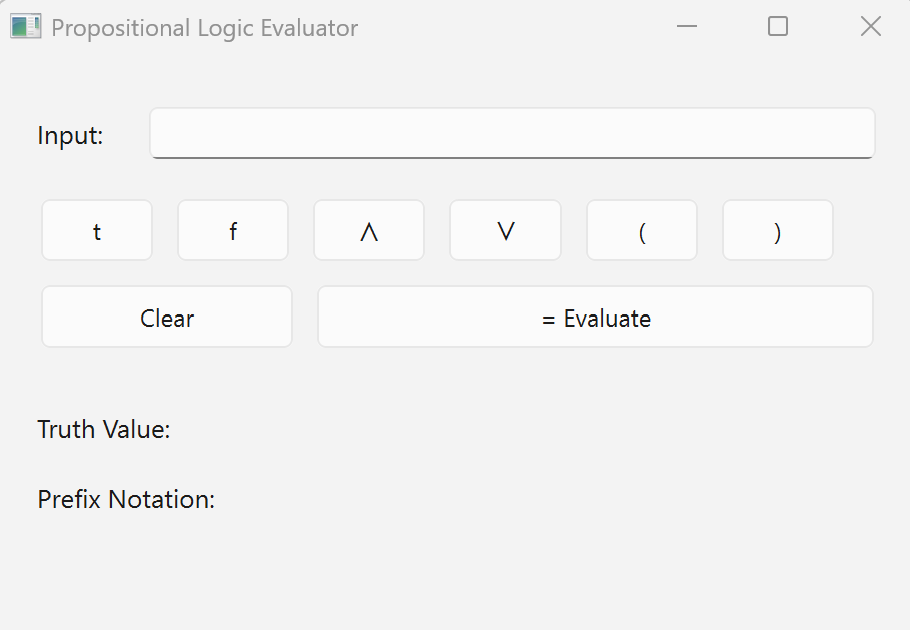
\includegraphics[width=\textwidth]{gui-preview.png}
    \caption{Empty GUI on launch}
    \label{fig:gui_preview}
\end{subfigure}
\hfill
\begin{subfigure}[t]{0.48\textwidth}
    \centering
    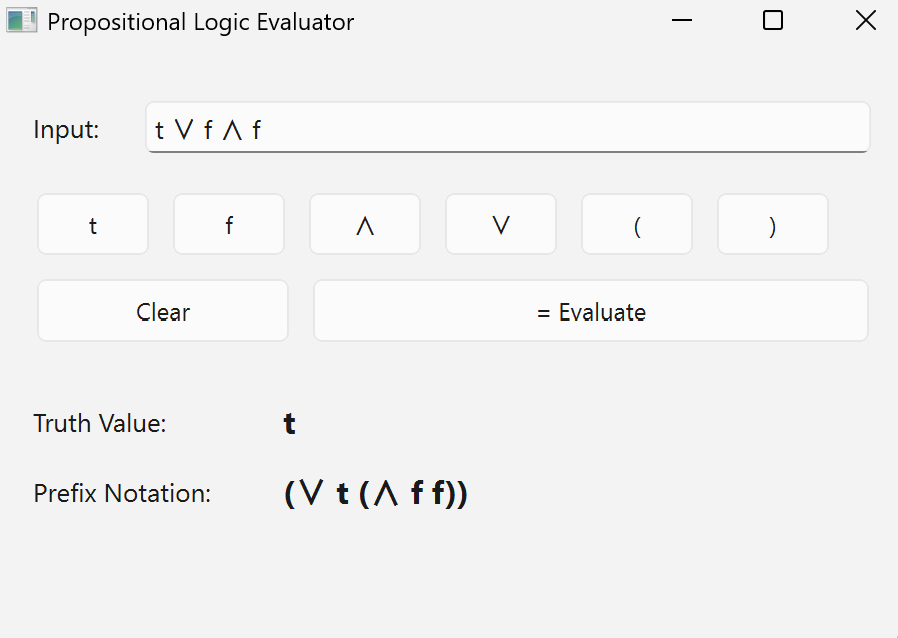
\includegraphics[width=\textwidth]{order-precedence.png}
    \caption{Operator precedence: \texttt{t $\vee$ f $\wedge$ f $\Rightarrow$ t}}
    \label{fig:order_precedence}
\end{subfigure}

\vspace{0.5em}

\begin{subfigure}[t]{0.48\textwidth}
    \centering
    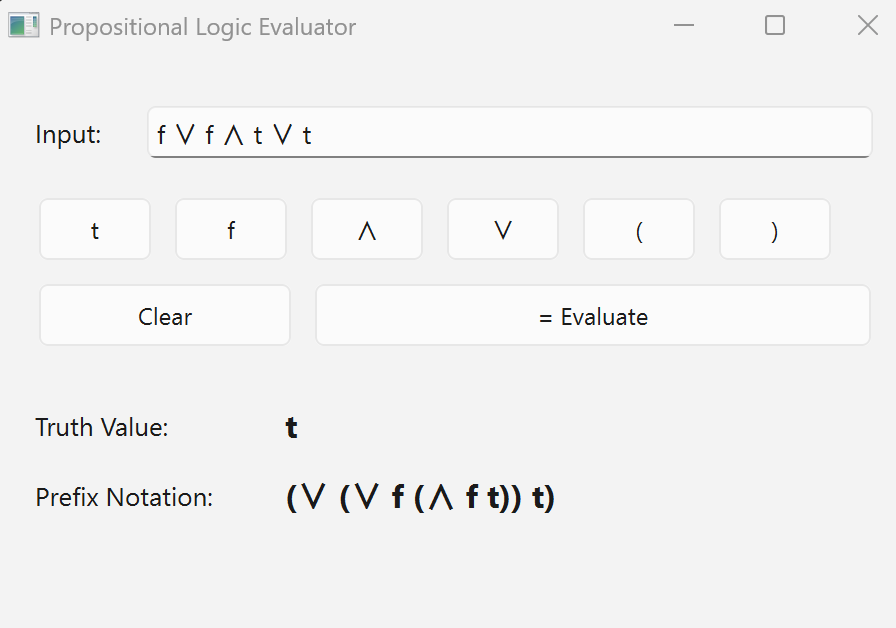
\includegraphics[width=\textwidth]{precedence-leftassoc.png}
    \caption{Left-associativity: \texttt{f $\vee$ f $\wedge$ t $\vee$ t $\Rightarrow$ t}}
    \label{fig:precedence_leftassoc}
\end{subfigure}
\hfill
\begin{subfigure}[t]{0.48\textwidth}
    \centering
    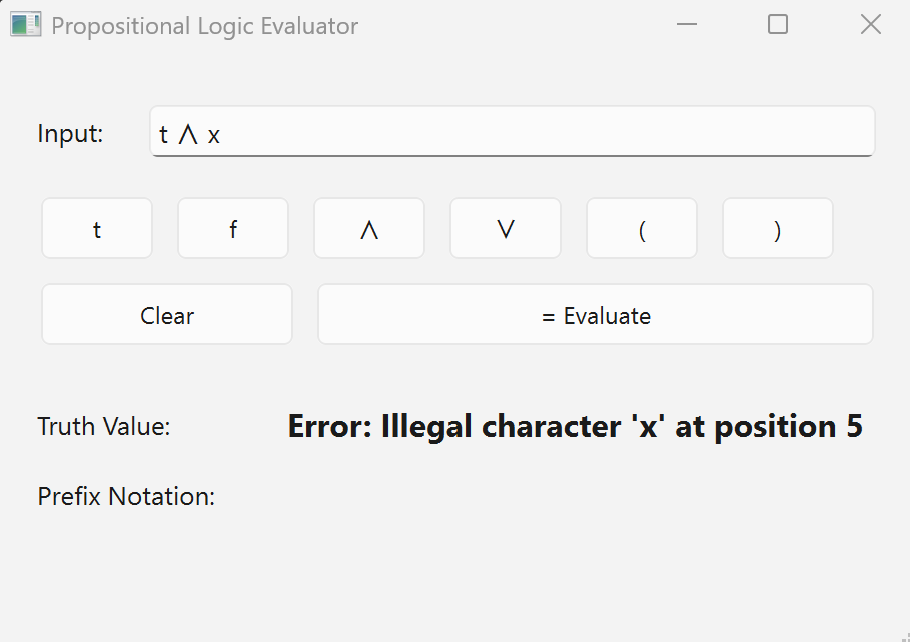
\includegraphics[width=\textwidth]{error-illegalchar.png}
    \caption{Error handling: illegal character \texttt{x}}
    \label{fig:error_illegalchar}
\end{subfigure}
\caption{Application screenshots --- GUI layout, operator precedence, left-associativity, and error handling}
\label{fig:screenshots}
\end{figure}

\subsection{GUI Interaction Flow}

When the user clicks \textbf{Evaluate}, a fresh lexer and parser are instantiated. The input text is tokenised, parsed into an AST, and the AST's \texttt{run()} and \texttt{prefix()} methods produce the truth value and prefix string, respectively.  If the input is invalid, an error message is displayed instead.


\section{Integration of Parser and Translation}

The assignment requires both a truth value and a prefix notation string from a single input.  Rather than embedding computation inside grammar rules, this implementation uses the AST as an \textbf{intermediate representation} that decouples parsing from downstream processing:

\begin{enumerate}
    \item \textbf{Parser $\rightarrow$ AST:} Each grammar rule's semantic action (Listing~\ref{lst:grammar_rules}) constructs an AST node during bottom-up reduction --- a form of \emph{syntax-directed translation}~\citep{aho2006compilers}.
    \item \textbf{AST $\rightarrow$ Truth value:} \texttt{run()} performs a post-order traversal (Listing~\ref{lst:run}).
    \item \textbf{AST $\rightarrow$ Prefix string:} \texttt{prefix()} performs a pre-order traversal (Listing~\ref{lst:prefix}).
\end{enumerate}

Because both traversals operate on the \emph{same} tree, the expression is parsed only once:

\begin{lstlisting}[caption={Pipeline integration in \texttt{MainWindow.evaluate()}}, label={lst:integration}]
result = parser.parse(lexer.tokenize(input_text))  # parse once
truth_value = result.run()                          # traversal 1
prefix_str  = result.prefix()                       # traversal 2
\end{lstlisting}

This clean separation means adding a new output format (e.g.\ postfix notation) requires only a new traversal method --- the parser and grammar remain unchanged.

    \chapter{TESTING AND VERIFICATION}

\section{Test Cases}

All six required test cases were executed and verified against expected outputs. Table~\ref{table:test_results} presents the complete results.

\begin{table}[H]
\centering
\caption{Test case results --- all cases pass}
\label{table:test_results}
\begin{tabular}{@{}clcccc@{}}
\toprule
\# & Input & Expected Value & Actual Value & Expected Prefix & Actual Prefix \\
\midrule
1 & \texttt{t}                          & \texttt{t} & \texttt{t} & \texttt{t}                              & \texttt{t} \\
2 & \texttt{f}                          & \texttt{f} & \texttt{f} & \texttt{f}                              & \texttt{f} \\
3 & \texttt{t $\wedge$ f}               & \texttt{f} & \texttt{f} & \texttt{($\wedge$ t f)}                 & \texttt{($\wedge$ t f)} \\
4 & \texttt{t $\vee$ f}                 & \texttt{t} & \texttt{t} & \texttt{($\vee$ t f)}                   & \texttt{($\vee$ t f)} \\
5 & \texttt{t $\vee$ f $\wedge$ f}      & \texttt{t} & \texttt{t} & \texttt{($\vee$ t ($\wedge$ f f))}      & \texttt{($\vee$ t ($\wedge$ f f))} \\
6 & \texttt{(t $\vee$ f) $\wedge$ f}    & \texttt{f} & \texttt{f} & \texttt{($\wedge$ ($\vee$ t f) f)}      & \texttt{($\wedge$ ($\vee$ t f) f)} \\
\bottomrule
\end{tabular}
\end{table}

\textbf{Result: All 6 test cases pass.} Expected and actual outputs match for both truth value and prefix notation.

\section{Detailed Analysis of Key Test Cases}

\subsection{Test Case 5: \texttt{t $\vee$ f $\wedge$ f} --- Operator Precedence}

This test case validates that $\wedge$ (AND) binds tighter than $\vee$ (OR).

\textbf{Without precedence rules} (left-to-right), the expression would be parsed as $(\texttt{t} \vee \texttt{f}) \wedge \texttt{f} = \texttt{f}$.

\textbf{With correct precedence} ($\wedge$ before $\vee$), the expression is parsed as $\texttt{t} \vee (\texttt{f} \wedge \texttt{f}) = \texttt{t}$.

The actual output \texttt{t} with prefix \texttt{($\vee$ t ($\wedge$ f f))} confirms that the parser correctly applies $\wedge > \vee$ precedence. The AST for this case is shown in Figure~\ref{fig:ast_example}.

\subsection{Test Case 6: \texttt{(t $\vee$ f) $\wedge$ f} --- Parenthesised Grouping}

This test case validates that explicit parentheses override the default precedence.

\textbf{Default precedence} would evaluate $\texttt{f} \wedge \texttt{f}$ first. But the parentheses force $\texttt{t} \vee \texttt{f}$ to be grouped first:
\begin{equation}
(\texttt{t} \vee \texttt{f}) \wedge \texttt{f} \;=\; \texttt{t} \wedge \texttt{f} \;=\; \texttt{f}
\end{equation}

The actual output \texttt{f} with prefix \texttt{($\wedge$ ($\vee$ t f) f)} confirms correct parenthesised grouping. The AST for this case is shown in Figure~\ref{fig:ast_paren}.

\section{Walkthrough: Complete Pipeline Execution}

This section walks through the complete execution pipeline for the input \texttt{t $\vee$ f $\wedge$ f}, demonstrating how each component transforms the data.

\textbf{Step 1 --- Lexical Analysis:}
\begin{center}
\texttt{t $\vee$ f $\wedge$ f} $\;\longrightarrow\;$ \texttt{TRUE\; OR\; FALSE\; AND\; FALSE}
\end{center}

\textbf{Step 2 --- Parsing (LALR(1) shift-reduce):}
The parser processes the token stream as shown in Table~\ref{table:parse_trace} (Chapter 4), building the AST bottom-up through 11 shift/reduce steps.

\textbf{Step 3 --- AST Construction:}
The resulting AST is shown in Figure~\ref{fig:ast_example} (Chapter 4): a $\vee$ root with \texttt{t} as the left child and a $\wedge$ subtree as the right child.

\textbf{Step 4 --- Evaluation (\texttt{run()}):}
Bottom-up traversal:
\begin{align}
\texttt{f} \wedge \texttt{f} &= \texttt{f} \\
\texttt{t} \vee \texttt{f} &= \texttt{t}
\end{align}

\textbf{Step 5 --- Translation (\texttt{prefix()}):}
Pre-order traversal:
\begin{equation}
(\vee\; \texttt{t}\; (\wedge\; \texttt{f}\; \texttt{f}))
\end{equation}

\textbf{Final Output:}
\begin{center}
Truth Value $=$ \texttt{t}, \quad Prefix Notation $=$ \texttt{($\vee$ t ($\wedge$ f f))}
\end{center}

\section{Error Handling}

The evaluator handles invalid input at three levels:

\begin{itemize}
    \item \textbf{Lexical errors:} If the input contains an unrecognised character (e.g.\ \texttt{x}), the lexer's \texttt{error()} method reports the illegal character and its position, then advances past it to continue scanning.
    \item \textbf{Syntax errors:} If the token stream does not conform to the grammar (e.g.\ \texttt{t t} or \texttt{t $\wedge$}), the LALR(1) parser returns \texttt{None}, and the GUI displays an error message instead of a result.
    \item \textbf{Runtime exceptions:} Any unexpected exception during the pipeline is caught by the \texttt{evaluate()} method, and the error message is displayed in the truth value output field.
\end{itemize}

This layered approach ensures the application never crashes on malformed input and always provides feedback to the user.

    \chapter{CONCLUSION}

This report presented a \textbf{Propositional Logic Evaluator} that applies classical compiler front-end techniques to evaluate expressions over truth values (\texttt{t}, \texttt{f}) with conjunction ($\wedge$) and disjunction ($\vee$). The system follows a four-stage pipeline --- lexical analysis, LALR(1) parsing (via SLY~\citep{beazley2023sly}), post-order AST evaluation, and pre-order prefix translation --- producing both the evaluated truth value and an equivalent prefix notation string from a single parse~\citep{aho2006compilers}. An interactive PySide6 GUI with dual Unicode/ASCII input modes completes the implementation. All six required test cases pass correctly (Chapter~4, Table~\ref{table:test_results}).

Three design choices merit emphasis: using an \textbf{LALR(1) parser generator} keeps the grammar declarative and aligned with formal BNF notation; constructing an \textbf{AST as an intermediate representation} decouples parsing from downstream processing, enabling independent tree traversals for evaluation and translation without re-parsing; and producing \textbf{fully parenthesised prefix notation} ensures unambiguous output regardless of operator precedence. Future extensions could include additional connectives ($\neg$, $\rightarrow$, $\leftrightarrow$), named propositional variables, automatic truth table generation, and step-by-step evaluation visualisation.


    % ---- References ----
    \newpage
    \pagestyle{plain}
    \phantomsection
    \addcontentsline{toc}{chapter}{REFERENCES}
    \renewcommand{\bibsection}{%
      \chapter*{REFERENCES}%
    }
    \bibliographystyle{plainnat}
    \bibliography{references}

    % ---- Appendices ----
    \newpage
    \chapter*{APPENDIX A: SOURCE CODE AVAILABILITY}
\addcontentsline{toc}{chapter}{APPENDIX A: SOURCE CODE AVAILABILITY}

The complete source code for the Propositional Logic Evaluator is publicly available on GitHub:

\begin{center}
\textbf{\url{https://github.com/limhpone/125970-Assignment-1-Propositional-Logic-Evaluator-PLC.git}}
\end{center}

\noindent A video walkthrough demonstrating the evaluator in action is available on YouTube:

\begin{center}
\textbf{\url{https://youtu.be/jVUvnhstTXY}}
\end{center}

The repository contains the following components:

\begin{itemize}
    \item \textbf{Lexical analyser} (\texttt{components/lexica.py}) --- tokenises input expressions into \texttt{TRUE}, \texttt{FALSE}, \texttt{AND}, \texttt{OR}, \texttt{LPAREN}, \texttt{RPAREN}
    \item \textbf{LALR(1) parser} (\texttt{components/parsers.py}) --- parses token streams and builds an abstract syntax tree
    \item \textbf{AST node classes} (\texttt{components/ast/statement.py}) --- \texttt{Expression\_bool} (leaf) and \texttt{Expression\_logic} (binary) with \texttt{run()} and \texttt{prefix()} methods
    \item \textbf{GUI layout} (\texttt{components/ui.py}) --- PySide6 interface definition
    \item \textbf{Entry point} (\texttt{main.py}) --- GUI window creation and pipeline orchestration
\end{itemize}

\section*{How to Run}

\begin{enumerate}
    \item Clone the repository:
    \begin{verbatim}
    git clone https://github.com/limhpone/
        125970-Assignment-1-Propositional-Logic-Evaluator-PLC.git
    \end{verbatim}
    \item Install dependencies using \texttt{uv}:
    \begin{verbatim}
    uv sync
    \end{verbatim}
    \item Run the application:
    \begin{verbatim}
    cd src/125970eval
    uv run main.py
    \end{verbatim}
\end{enumerate}

\section*{Source Code Listings}

The key implementation files are reproduced below for reference.

\subsection*{A.1 Lexical Analyser --- \texttt{components/lexica.py}}

\begin{lstlisting}[language=Python]
from sly import Lexer

class PropLogicLexer(Lexer):
    tokens = { TRUE, FALSE, AND, OR, LPAREN, RPAREN }

    ignore = ' \t'

    AND    = r'[∧&]'
    OR     = r'[∨|]'
    LPAREN = r'\('
    RPAREN = r'\)'
    TRUE   = r't'
    FALSE  = r'f'

    @_(r'\n+')
    def ignore_newline(self, t):
        self.lineno += t.value.count('\n')

    def error(self, t):
        bad = t.value[0]
        self.index += 1
        raise ValueError(
            f"Illegal character '{bad}' "
            f"at position {self.index}")
\end{lstlisting}

\subsection*{A.2 Parser --- \texttt{components/parsers.py}}

\begin{lstlisting}[language=Python]
from components.lexica import PropLogicLexer
from components.ast.statement import (Expression, Expression_bool,
                                      Expression_logic, Operations)
from sly import Parser

class PropLogicParser(Parser):
    debugfile = 'parser.out'
    start = 'statement'
    tokens = PropLogicLexer.tokens
    precedence = (
        ('left', OR),
        ('left', AND),
    )

    @_('expr')
    def statement(self, p):
        return p.expr

    @_('expr OR expr')
    def expr(self, p) -> Expression:
        return Expression_logic(Operations.OR, p.expr0, p.expr1)

    @_('expr AND expr')
    def expr(self, p) -> Expression:
        return Expression_logic(Operations.AND, p.expr0, p.expr1)

    @_('LPAREN expr RPAREN')
    def expr(self, p) -> Expression:
        return p.expr

    @_('TRUE')
    def expr(self, p) -> Expression:
        return Expression_bool(True)

    @_('FALSE')
    def expr(self, p) -> Expression:
        return Expression_bool(False)
\end{lstlisting}

\subsection*{A.3 AST Node Classes --- \texttt{components/ast/statement.py}}

\begin{lstlisting}[language=Python]
from enum import Enum
from abc import ABC, abstractmethod

class Operations(Enum):
    AND = 0
    OR = 1

class Expression(ABC):
    @abstractmethod
    def __init__(self) -> None:
        self.value = None

    @abstractmethod
    def run(self):
        pass

    @abstractmethod
    def prefix(self) -> str:
        pass

class Expression_bool(Expression):
    def __init__(self, value: bool) -> None:
        self.value: bool = value

    def run(self):
        return self.value

    def prefix(self) -> str:
        return 't' if self.value else 'f'

class Expression_logic(Expression):
    def __init__(self, operation: Operations,
                 left: Expression,
                 right: Expression) -> None:
        self.operation = operation
        self.left = left
        self.right = right
        self.value = None

    def run(self):
        left_val = self.left.run()
        right_val = self.right.run()
        if self.operation == Operations.AND:
            self.value = left_val and right_val
        elif self.operation == Operations.OR:
            self.value = left_val or right_val
        return self.value

    def prefix(self) -> str:
        op_str = '∧' if self.operation == Operations.AND else '∨'
        return (f"({op_str} {self.left.prefix()} "
                f"{self.right.prefix()})")
\end{lstlisting}

\subsection*{A.4 Main Entry Point --- \texttt{main.py}}

\begin{lstlisting}[language=Python]
import sys
from PySide6.QtWidgets import QApplication, QMainWindow
from components.lexica import PropLogicLexer
from components.parsers import PropLogicParser
from components.ui import Ui_MainWindow

class MainWindow(QMainWindow):
    def __init__(self):
        super(MainWindow, self).__init__()
        self.ui = Ui_MainWindow()
        self.ui.setupUi(self)

        self.ui.button_t.clicked.connect(lambda: self.push("t"))
        self.ui.button_f.clicked.connect(lambda: self.push("f"))
        self.ui.button_and.clicked.connect(
            lambda: self.push(" \u2227 "))
        self.ui.button_or.clicked.connect(
            lambda: self.push(" \u2228 "))
        self.ui.button_lparen.clicked.connect(
            lambda: self.push("("))
        self.ui.button_rparen.clicked.connect(
            lambda: self.push(")"))
        self.ui.button_clear.clicked.connect(self.clear)
        self.ui.button_equal.clicked.connect(self.evaluate)

    def push(self, text: str):
        current_text = self.ui.input_text.text()
        self.ui.input_text.setText(f"{current_text}{text}")

    def clear(self):
        self.ui.input_text.setText("")
        self.ui.output_value.setText("")
        self.ui.output_prefix.setText("")

    def evaluate(self):
        lexer = PropLogicLexer()
        parser = PropLogicParser()
        input_text = self.ui.input_text.text()
        try:
            result = parser.parse(lexer.tokenize(input_text))
            if result is not None:
                truth_value = result.run()
                self.ui.output_value.setText(
                    't' if truth_value else 'f')
                self.ui.output_prefix.setText(result.prefix())
            else:
                self.ui.output_value.setText(
                    "Error: Invalid expression")
                self.ui.output_prefix.setText("")
        except ValueError as e:
            self.ui.output_value.setText(f"Error: {e}")
            self.ui.output_prefix.setText("")
        except Exception as e:
            self.ui.output_value.setText(f"Error: {e}")
            self.ui.output_prefix.setText("")

if __name__ == "__main__":
    app = QApplication(sys.argv)
    window = MainWindow()
    window.show()
    sys.exit(app.exec())
\end{lstlisting}


\end{document}
